\documentclass{article}
\usepackage[utf8]{inputenc}
\usepackage{geometry}
\usepackage{hyperref}
 \geometry{
 a4paper,
 total={170mm,257mm},
 left=20mm,
 top=20mm,
 }
 \usepackage{graphicx}
 \usepackage{titling}

\title{\textbf{Assignment 3 Part 1:} Probabilistic Reasoning}
\author{Ehsan, Goldstein}
\date{April 2023}
 
 \usepackage{fancyhdr}
\fancypagestyle{plain}{%  the preset of fancyhdr 
    \fancyhf{} % clear all header and footer fields
    \fancyfoot[C]{\thepage}
    \fancyhead[L]{CS440 Intro to AI}
    \fancyhead[R]{\theauthor}
}
\makeatletter
\def\@maketitle{%
  \newpage
  \null
  \vskip 1em%
  \begin{center}%
  \let \footnote \thanks
    {\LARGE \@title \par}%
    \vskip 1em%
    %{\large \@date}%
  \end{center}%
  \par
  \vskip 1em}
\makeatother

\usepackage{lipsum}  
\usepackage{cmbright}

\begin{document}

\maketitle

\noindent\begin{tabular}{@{}ll}
    \textbf{Submitted By: }Brandon Goldstein (bbg17), Taqiya Ehsan (te137)\\
     \textbf{Date:} 14 April 2023
\end{tabular}

\subsection*{Problem 1}
\subsubsection*{a} P(A, B, C, D, E) = P(A) * P(B) * P(C) * P(D$\vert$A,B) * P(E$\vert$B,C) \\

\noindent
P(A = true, B = true, C = true, D = true, E = true) \\
\indent 
= P(A = true) * P(B = true) * P(C = true) * P(D = true $\vert$ A = true $\land$ B = true) * P(E = true $\vert$ B = true $\land$ C = true) \\ 
\indent
= 0.2 * 0.5 * 0.8 * 0.1 * 0.3 \\
\indent 
= \textbf{0.0024}

\subsubsection*{b} P(A, B, C, D, E) = P(A) * P(B) * P(C) * P(D$\vert$A,B) * P(E$\vert$B,C) \\

\noindent
P(A = false, B = false, C = false, D = false, E = false) \\
\indent 
= P(A = false) * P(B = false) * P(C = false) * P(D = false $\vert$ A = false $\land$ B = false) * P(E = false $\vert$ B = false $\land$ C = false) \\
\indent
= 0.8 * 0.5 * 0.2 * 0.1 * 0.8 \\
\indent 
= \textbf{0.0064}

\subsubsection*{c} P(A = false $\vert$ B = true, C = true, D = true, E = true) = $\frac{P(A = false, B = true, C = true, D = true, E = true)}{\sum_{A} P(B = true, C = true, D = true, E = true)}$ \\

\noindent
For brevity we denote P(A = false, B = true, C = true, D = true, E = true) as P($\neg$A, B, C, D, E) and P(A = true, B = true, C = true, D = true, E = true) as P(A, B, C, D, E)\\

\noindent
We can denote the denominator as a constant $\alpha$. So the expression stands - \\
P(A = false $\vert$ B = true, C = true, D = true, E = true) = $\alpha$ * P($\neg$A, B, C, D, E) \\ where, $\alpha$ = $\frac{1}{\sum_{A} P(B, C, D, E)}$ \\

\noindent
P($\neg$A, B, C, D, E) \\
\indent
= P($\neg$A) * P(B) * P(C) P(D $\vert$ B $\land$ $\neg$A) * P(D $\vert$ B $\land$ C) \\ 
\indent 
= 0.8 * 0.5 * 0.8 * 0.6 * 0.3 \\
\indent 
= 0.0576 \\

\noindent
$\sum_{A} P(B, C, D, E)$ \\ 
\indent
= P(A, B, C, D, E) + P($\neg$A, B, C, D, E) \\
\indent 
= 0.0576 + 0.0024 (from part a)\\
\indent 
= \textbf{$\frac{3}{50}$} \\

\noindent
So, $\alpha$ = \textbf{$\frac{50}{3}$}\\

\noindent
Therefore, \\
P(A = false $\vert$ B = true, C = true, D = true, E = true) = $\frac{50}{3}$ * 0.0576 = \textbf{0.96}

\subsection*{Problem 2}
\subsubsection*{a} P(B $\vert$ J = true, M = true) = $\frac{P(B, J, M)}{P(J, M)}$ \\ 

\noindent 
Let, $\alpha$ = $\frac{1}{P(J, M)}$ \\

\noindent
P(J, M) \\ 

\indent 
= $\sum_{B}\sum_{E}\sum_{A}P(B)P(E)P(A \vert B, E)P(J \vert A)P(M \vert A)$ \\ 

\indent 
= $\sum_{A}P(J \vert A)P(M \vert A)\sum_{E}P(E)\sum_{B}P(B)P(A \vert B, E)$ \\

\indent 
= $\sum_{A}P(J \vert A)P(M \vert A)\sum_{E}P(E) * [0.001 
    \left(\begin{array}{cc} 
        0.95 & 0.05 \\ 
        0.94 & 0.06 
        \end{array}\right)
+ 0.999
    \left(\begin{array}{cc} 
        0.29 & 0.71 \\ 
        0.001 & 0.999 
        \end{array}\right)]$ \\ 

\indent 
= $\sum_{A}P(J \vert A)P(M \vert A)\sum_{E}P(E) 
    \left(\begin{array}{cc} 
        0.29066 & 0.70934 \\ 
        0.001939 & 0.998061 
        \end{array}\right)$ \\ 

\indent 
= $\sum_{A}P(J \vert A)P(M \vert A)* 0.002 
    \left(\begin{array}{c} 
        0.29066 \\ 
        0.70934
        \end{array}\right) + 0.998 
    \left(\begin{array}{c} 
        0.001939 \\ 
        0.998061 
        \end{array}\right)$ \\ 

\indent 
= $\sum_{A}P(J \vert A)P(M \vert A) * 
    \left(\begin{array}{c} 
        0.002516442 \\ 
        0.997483558 
        \end{array}\right)$ \\ 

\indent 
= $0.9 * 0.7 * 0.002516442 + 0.05 * 0.01 * 0.997483558$ \\

\indent 
= 0.002084100239 \\
\\

\noindent
P(B, J, M) \\ 

\indent 
= $\sum_{E}\sum_{A}P(B)P(E)P(A \vert B, E)P(J \vert A)P(M \vert A)$ \\ 

\indent 
= $P(B)\sum_{E}P(E)\sum_{A}P(A \vert B, E)P(J \vert A)P(M \vert A)$ \\ 

\indent 
= $P(B)\sum_{E}P(E)* (0.9 * 0.7 * 
\left(\begin{array}{cc} 
        0.95 & 0.29 \\ 
        0.94 & 0.001 
        \end{array}\right) + 
0.5 * 0.01 * 
\left(\begin{array}{cc} 
        0.05 & 0.71 \\ 
        0.06 & 0.999 
        \end{array}\right))$ \\ 

\indent 
= $P(B)\sum_{E}P(E) * 
    \left(\begin{array}{cc} 
        0.598525 & 0.183055 \\ 
        0.59223 & 0.0011295 
        \end{array}\right)$ \\ 

\indent 
= $P(B)*(0.002 * 
    \left(\begin{array}{c} 
        0.598525\\ 
        0.183055 
        \end{array}\right) + 
    0.998 * 
    \left(\begin{array}{c} 
        0.59223 \\ 
        0.0011295
        \end{array}\right))$ \\ 

\indent 
= $\left(\begin{array}{c} 
        0.001 * 0.59224259 \\ 
        0.999 * 0.001493341
        \end{array}\right)$\\ 

\indent 
= $\langle 0.00059224259, 0.001491857649 \rangle$ \\ 
\\

\noindent
P(B $\vert$ J, M) \\

\indent
= $\frac{P(B, J, M)}{P(J, M)}$ \\

\indent
= $\alpha$ * P(B, J, M) \\

\indent 
= $\frac{1}{0.002084100239}*\langle 0.00059224259, 0.001491857649 \rangle$ \\ 

\indent 
= $\langle 0.284, 0.716 \rangle$\\ 

\noindent 
Hence, if both John and Mary call, the probability that Burglary happened is \textbf{0.284} and not happened is \textbf{0.716}. 

\subsubsection*{b}
\textbf{Inference by Enumeration}: To apply this method for a chain Bayesian network, we would construct an enumeration tree. As $X_i$ is Boolean variable for all $i$, the enumeration tree is composed of two complete binary trees, both with depth $n-2$. We then use depth-first search, as in class, to parse the enumeration tree and complete the method. By the properties of depth-first search, parsing the constructed enumeration tree can be done with time complexity \textbf{O($2^{n}$)}. So, the complexity of computing $P(X_1 | X_n = true)$ using enumeration is \textbf{O($2^{n}$)}.  \\

\noindent
\textbf{Inference by Variable Elimination}: We can use factors for this method, where a factor $f_i$ is a matrix indexed by the values of its argument variables (as in class). Note, by construction, the first step of variable elimination is the following ($\alpha$ is the normalization factor): \\

\noindent
$P(X_1 | X_n = true) = \alpha P(X_1)... \sum_{X_{n-2}}P(X_{n-2} | X_{n-3}) \sum_{X_{n-1}}P(X_{n-1} | X_{n-2})P(X_n = true | X_{n-1})$ \\

\noindent
$P(X_1 | X_n = true) = \alpha P(X_1)... \sum_{X_{n-2}}P(X_{n-2} | X_{n-3}) \sum_{X_{n-1}}f_{X_{n-1}}(X_{n-1}, X_{n-2})f_{X_n}(X_{n-1})$ \\

\noindent
$P(X_1 | X_n = true) = \alpha P(X_1)... \sum_{X_{n-2}}P(X_{n-2} | X_{n-3})f_{X_{n-1}, X_n}(X_{n-2})$ \\

\noindent 
Notice how the conclusion of this step produces an expression of the same form as the original problem, but with $n-1$ variables instead of $n$ variables. Critically, the first step (as shown above) can be performed in constant time (\textbf{O(1)}), as the factors never involve more than 2 variables as arguments (this is a result of the construction of the problem as a chain). As the first step can be done in constant time and leads to a problem of the same form with $n-1$ variables instead of $n$ variables, it follows by induction on $n$ that the complexity of computing $P(X_1 | X_n = true)$ using variable elimination is \textbf{O(n)}.

\subsection*{Problem 3}

\subsubsection*{a}
\begin{figure}[!htbp]
\centering
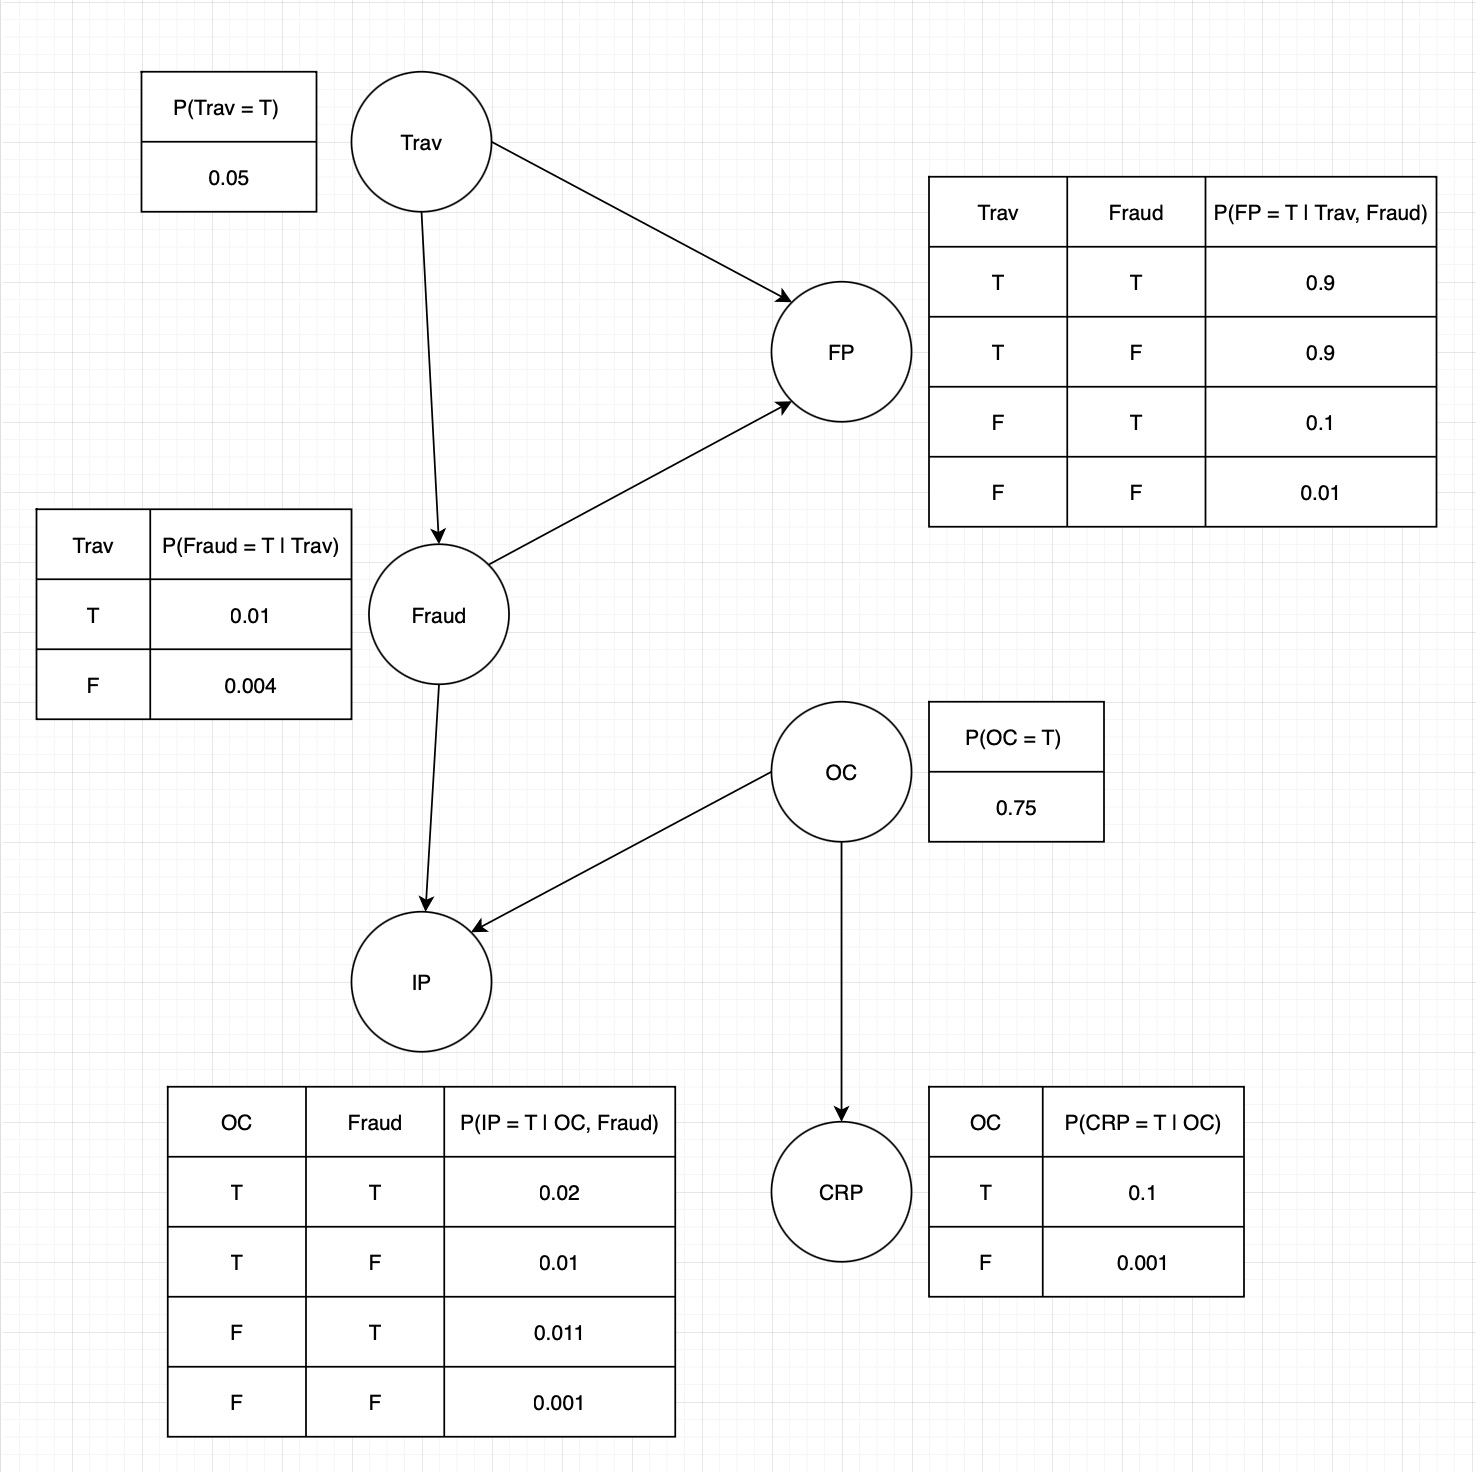
\includegraphics[width=0.5\textwidth, height=0.5\textheight,keepaspectratio]{Network_and_Probabilities}
\caption{Bayes Network and Conditional Probability Tables}
\end{figure}
\subsubsection*{b}
$P(Fraud = T) = \sum_{Trav} P(Fraud = T | Trav)P(Trav) = ((0.01)(0.05)+(0.004)(0.95)) = 0.0043$
\newline
\newline
\noindent
$P(Fraud = T | FP = T, IP = F, CRP = T) = \alpha P(Fraud = T, FP = T, IP = F, CRP = T)$
\newline
\newline
$\alpha P(Fraud = T, FP = T, IP = F, CRP = T) = \alpha \sum_{Trav} \sum_{OC} P(Fraud = T, FP = T, IP = F, CRP = T, Trav, OC)$
\newline
\newline
$\alpha \sum_{Trav} \sum_{OC} P(Fraud = T, FP = T, IP = F, CRP = T, Trav, OC) = \alpha \sum_{Trav} \sum_{OC} P(Trav)P(OC)P(CRP = T | OC)P(Fraud = T | Trav)P(FP = T | Fraud = T, Trav)P(IP = F | Fraud = T, OC)$
\newline
\newline
$\alpha \sum_{Trav} \sum_{OC} P(Trav)P(OC)P(CRP = T | OC)P(Fraud = T | Trav)P(FP = T | Fraud = T, Trav)P(IP = F | Fraud = T, OC) = \alpha \sum_{Trav} P(Trav)P(Fraud = T | Trav)P(FP = T | Fraud = T, Trav) \sum_{OC} P(OC)P(CRP = T | OC)P(IP = F | Fraud = T, OC)$
\newline
\newline
$\sum_{OC} P(OC)P(CRP = T | OC)P(IP = F | Fraud = T, OC) = ((0.75)(0.1)(0.98) + (0.25)(0.001)(0.989)) = 0.07374725$
\newline
\newline
$\alpha \sum_{Trav} P(Trav)P(Fraud = T | Trav)P(FP = T | Fraud = T, Trav) \sum_{OC} P(OC)P(CRP = T | OC)P(IP = F | Fraud = T, OC) = \alpha (0.07374725) \sum_{Trav} P(Trav)P(Fraud = T | Trav)P(FP = T | Fraud = T, Trav)$
\newline
\newline
$\sum_{Trav} P(Trav)P(Fraud = T | Trav)P(FP = T | Fraud = T, Trav) = ((0.05)(0.01)(0.9) + (0.95)(0.004)(0.1)) = 0.00083$
\newline
\newline
$\alpha (0.07374725) \sum_{Trav} P(Trav)P(Fraud = T | Trav)P(FP = T | Fraud = T, Trav) = \alpha (0.07374725)(0.00083) = \alpha (0.0000612102175)$
\newline
\newline
$\alpha = 1/(P(Fraud = T, FP = T, IP = F, CRP = T) + P(Fraud = F, FP = T, IP = F, CRP = T))$
\newline
\newline
$P(Fraud = T, FP = T, IP = F, CRP = T) = 0.0000612102175$
\newline
\newline
$P(Fraud = F, FP = T, IP = F, CRP = T) = \sum_{Trav} \sum_{OC} P(Fraud = F, FP = T, IP = F, CRP = T, Trav, OC)$
\newline
\newline
$\sum_{Trav} \sum_{OC} P(Fraud = F, FP = T, IP = F, CRP = T, Trav, OC) = \sum_{Trav} \sum_{OC} P(Trav)P(OC)P(CRP = T | OC)P(Fraud = F | Trav)P(FP = T | Fraud = F, Trav)P(IP = F | Fraud = F, OC)$
\newline
\newline
$\sum_{Trav} \sum_{OC} P(Trav)P(OC)P(CRP = T | OC)P(Fraud = F | Trav)P(FP = T | Fraud = F, Trav)P(IP = F | Fraud = F, OC) = \sum_{Trav} P(Trav)P(Fraud = F | Trav)P(FP = T | Fraud = F, Trav) \sum_{OC} P(OC)P(CRP = T | OC)P(IP = F | Fraud = F, OC)$
\newline
\newline
$\sum_{OC} P(OC)P(CRP = T | OC)P(IP = F | Fraud = F, OC) = ((0.75)(0.1)(0.99) + (0.25)(0.001)(0.999)) = 0.07449975$
\newline
\newline
$\sum_{Trav} P(Trav)P(Fraud = F | Trav)P(FP = T | Fraud = F, Trav) \sum_{OC} P(OC)P(CRP = T | OC)P(IP = F | Fraud = F, OC) = (0.07449975)\sum_{Trav} P(Trav)P(Fraud = F | Trav)P(FP = T | Fraud = F, Trav)$
\newline
\newline
$\sum_{Trav} P(Trav)P(Fraud = F | Trav)P(FP = T | Fraud = F, Trav) = ((0.05)(0.99)(0.9) + (0.95)(0.996)(0.01)) = 0.054012$
\newline
\newline
$(0.07449975)\sum_{Trav} P(Trav)P(Fraud = F | Trav)P(FP = T | Fraud = F, Trav) = (0.07449975)(0.054012) = 0.004023880497$
\newline
\newline
$P(Fraud = F, FP = T, IP = F, CRP = T) = 0.004023880497$
\newline
\newline
$1/(P(Fraud = T, FP = T, IP = F, CRP = T) + P(Fraud = F, FP = T, IP = F, CRP = T)) = 1/((0.0000612102175) + (0.004023880497)) = 244.792605572$
\newline
\newline
$\alpha = 244.792605572$
\newline
\newline
$\alpha (0.0000612102175) = (244.792605572)(0.0000612102175) = 0.0149838086294$
\newline
\newline
$P(Fraud = T | FP = T, IP = F, CRP = T) = 0.0149838086294$
\newline
\newline
The prior probability that the current transaction is a fraud ($P(Fraud = T)$) is \textbf{0.0043}.
\newline
The probability that the current transaction is a fraud once we have verified that it is a foreign transaction, but not an internet purchase and that the card holder purchased computer related accessories in the past week ($P(Fraud = T | FP = T, IP = F, CRP = T)$) is \textbf{0.0149838086294}. 

\end{document}